% -*- latex -*-
%-----------------------------------------------------------------------
%;  Copyright (C) 2014
%;  Associated Universities, Inc. Washington DC, USA.
%;
%;  This program is free software; you can redistribute it and/or
%;  modify it under the terms of the GNU General Public License as
%;  published by the Free Software Foundation; either version 2 of
%;  the License, or (at your option) any later version.
%;
%;  This program is distributed in the hope that it will be useful,
%;  but WITHOUT ANY WARRANTY; without even the implied warranty of
%;  MERCHANTABILITY or FITNESS FOR A PARTICULAR PURPOSE.  See the
%;  GNU General Public License for more details.
%;
%;  You should have received a copy of the GNU General Public
%;  License along with this program; if not, write to the Free
%;  Software Foundation, Inc., 675 Massachusetts Ave, Cambridge,
%;  MA 02139, USA.
%;
%;  Correspondence concerning AIPS should be addressed as follows:
%;          Internet email: aipsmail@nrao.edu.
%;          Postal address: AIPS Project Office
%;                          National Radio Astronomy Observatory
%;                          520 Edgemont Road
%;                          Charlottesville, VA 22903-2475 USA
%-----------------------------------------------------------------------
%Body of final AIPSletter for 31 December 2014

\documentclass[twoside]{article}
\usepackage{graphics}

\newcommand{\AIPRELEASE}{December 31, 2014}
\newcommand{\AIPVOLUME}{Volume XXXIV}
\newcommand{\AIPNUMBER}{Number 2}
\newcommand{\RELEASENAME}{{\tt 31DEC14}}
\newcommand{\OLDNAME}{{\tt 31DEC13}}
\newcommand{\NEWNAME}{{\tt 31DEC15}}
\newcommand{\Tsys}{${\rm T}_{\rm sys}$}

%macros and title page format for the \AIPS\ letter.
\input LET98.MAC

\newcommand{\MYSpace}{-11pt}

\normalstyle

\section{General developments in \AIPS}

\subsection{Reduction of VLA and ALMA data in \AIPS}

This \Aipsletter\ and those beginning in 2010 document numerous
improvements to \AIPS\ that enable full calibration of data from the
Karl G. Jansky VLA and most imaging operations as well.  The one
exception is the wide-band (bandwidth synthesis) deconvolution
algorithm (``MSMFS'') being developed in \CASA\ by Urvashi Rao
Venkata, for which there is no comparable function in \AIPS\@.
Calibrated $uv$ data may be exported from \AIPS\ in ``UVFITS'' format
for use in that program.  ALMA data may also be reduced in \AIPS,
although the package is not fully qualified to calibrate data from
linearly-polarized feeds.  See Appendix E of the \AIPS\ Cookbook,
available via the \AIPS\ web site, for details.

\subsection{\Aipsletter\ publication}

We have discontinued paper copies of the \Aipsletter\ other than for
libraries and NRAO staff.  The \Aipsletter\ will be available in
PostScript and pdf forms as always from the web site listed above and
will be shipped with all distributions of \AIPS\@.  It will be
announced on the bananas and mnj list servers and, usually, in the
NRAO e-News mailing.

\subsection{Current and future releases}

We have formal \AIPS\ releases on an annual basis.  We recommend a
full binary installation method for both the frozen and development
versions for MacIntosh OS/X (PPC and Intel chips), Solaris, and Linux
(32- and 64-bit) systems, but all architectures can do a full
installation from the source files.  If you develop \AIPS\ code
locally {\it or have system managers that forbid the use of\/} {\tt
  rsync} or {\tt cvs}, you will need to do a source-level
installation.  The current release is called \RELEASENAME\ and is now
``frozen.''  If you took a development copy of this version at some
earlier date, you should use the ``Midnight Job'' (MNJ) to bring it up
to date.  You need to run a MNJ only once in 2015 to convert your copy
of \RELEASENAME\ into the frozen version.  However, when patches to
\RELEASENAME\ are announced in 2015, you may apply them with the
MNJ\@.  This \Aipsletter\ is intended to advise you of corrections and
improvements in this release.

We have begun a new version, called \NEWNAME, which is now under
development by the \AIPS\ Group.  You may fetch and install a complete
copy of this version at any time.  Having fetched \NEWNAME, you may
update your installation whenever you want by running the MNJ\@.  This
uses {\tt cvs}, {\tt rsync}, and/or transaction files to copy all
changed text files and then to copy the binary files or to compile the
code selectively based on the code changes and compilations we have
done.  We expect users to take their source-only or binary version of
\NEWNAME\ \AIPS\ over the Internet (via \emph{anonymous} ftp).  Both
versions require you to copy the installation procedure {\tt
  install.pl} via {\tt ftp}; the source-only version also requires you
to ftp the 124-Mbyte {\tt   \NEWNAME.tar.gz} compressed tar file.
Linux sites will almost certainly have {\tt cvs} installed; other
sites may have installed it along with other GNU tools.  Secondary
MNJs will still be possible using {\tt ssh} or {\tt rcp} or NFS as
with previous releases.  We have found that {\tt cvs} works very well,
although it has one quirk. If a site modifies a file locally, but in
an \AIPS-standard directory, {\tt cvs} will detect the modification
and attempt to reconcile the local version with the NRAO-supplied
version.  This usually produces a file that will not compile or run as
intended.  Use a new name for the task or put a copy of the task and
its help file in a private disk area instead.

\AIPS\ is now copyright \copyright\ 1995 through 2014 by Associated
Universities, Inc., NRAO's parent corporation, but may be made freely
available under the terms of the Free Software Foundation's General
Public License (GPL)\@.  This means that User Agreements are no longer
required, that \AIPS\ may be obtained via anonymous ftp without
contacting NRAO, and that the software may be redistributed (and/or
modified), under certain conditions.  The full text of the GPL can be
found in the \texttt{15JUL95} \Aipsletter\ and is included with every
distribution in file {\tt \$AIPS\_ROOT/{\it release-name}/COPYING}\@.


\subsection{Installing a new version}

If compiling locally, new releases must be installed from the tar ball
for that release.  If using the binary installation, a full new
installation must also be done with {\tt rsync}.  The {\tt cvs} system
used in the MNJ requires this.  When installing a new \AIPS\ release
in a system that already has a previous release, we recommend that
{\tt install.pl} be used and that the previous release be left in
place, at least until the new installation has been verified.  If you
do this, then you will not have to re-edit the disk, printer, and tape
lists and can simply skip all those pages in the {\tt install.pl}
menus.  The old {\tt \$HOME/.AIPSRC} file may be left in place, but it
will need to be edited.  The lines giving the {\tt DOWNLOADED} and
{\tt UNPACKED} parameters should be cleared and the {\tt CCOMOPT} line
should be changed to point to the current release rather than the
previous one.  If you have made a special version of {\tt
  do\_daily.{\it host}}, you should preserve it under a new name and
restore it after the install.  If you have an odd set of \AIPS\
versions, the {\tt \$AIPS\_ROOT/AIPSPATH.*SH} files may need to be
edited after the install to set the desired versions.

{\tt 31DEC09} contains a change in the format of antenna files.
Previous releases will not understand the antenna coordinates for
arrays that were traditionally left-handed (VLBI primarily).  The
format change occurs automatically when any {\tt 31DEC09} or later
antenna-file specific code reads the file, after which older releases
will have difficulties.  Note that the only version which we patch for
major errors is \RELEASENAME; even \OLDNAME\ is no longer changed.

\section{Preview of coming attractions}

The \NEWNAME\ release already contains a few changes that we decided
were a bit risky or not needed in \RELEASENAME\@.  The low-level
Clean-component modeling routines were changed to allow an I
polarization model to be divided into the cross-hand polarization data
as well as the parallel-hand data.  {\tt UVSUB} offers this option
with {\tt OPCODE='DIV4'} and the option is, so far, not available in
any other task.  Interactive image histogram equalization. to replace
the non-functional tasks {\tt TVHXF} and {\tt TVHLD} (which requireD
an IIS Model 70), has appeared in {\tt 31DEC15} using the {\tt TVHLD}
name.

\section{Improvements of interest to users in \RELEASENAME}

We expect to continue publishing the \Aipsletter\ every six months
along with the annual releases.  There are a few new tasks and verbs
released in the last six months.  New task {\tt ACSCL} allows VLBI
amplitude adjustment after bandpass calibration and {\tt TVSAD} allows
interaction with the model fitting done by the ``search and destroy''
task {\tt SAD}\@.  New verb {\tt IMFITSET} provides similar TV
interaction to prepare the adverbs for the {\tt IMFIT} and {\tt JMFIT}
Gaussian-fitting tasks.  New verb {\tt GETDATE} returns a date string
in one of several user-selected formats.  A new data-reduction
pipeline procedure called {\tt VLBARUN}, located in a {\tt RUN} file
of the same name, was also released by Amy Mioduszewski.

In the first six months of \RELEASENAME\ the new tasks were {\tt
  BPWAY} to determine spectral channel-dependent $uv$ data weights,
{\tt DBAPP} to append multiple $uv$ data sets at once, {\tt CENTR} to
change the frequency reference pixel to the center of the spectrum,
{\tt HUINT} to adjust hue-intensity images interactively and then save
the result as image files, and {\tt MODSP} to compute model images of
spectral lines.  A set of {\tt RUN} files, under the general name {\tt
  TDEPEND}, was created to assist with imaging a time-dependent
source.  The cube model-fitting tasks {\tt XGAUS}, {\tt RMFIT}, and
{\tt ZEMAN} were given significant attention and a new \AIPS\ Memo was
written to document their usage.

Normally, bugs which appear in an \AIPS\ {\tt TST} version and then
are fixed in that same version before its release get little or no
discussion in the \Aipsletter\@.  Since a rather large number of sites
now install the {\tt TST} version of \AIPS\ during its development,
this is somewhat of an oversight.  We urge you to run the ``Midnight
Job'' at least once after \RELEASENAME\ is frozen to bring it up to
date and to fix all bugs of this sort.  We urge active sites to use
the MNJ and, when something odd occurs, to examine {\tt CHANGE.DOC}
using the cgi tool available from the \AIPS\ documentation web page
({\tt http://www.aips.nrao.edu/aipsdoc.html}).  Please do not
hesitate to contact us via the NRAO help desk ({\tt
  https://help.nrao.edu}) or via e-mail {\tt daip@nrao.edu} with any
questions or suspicions that there are problems.

\subsection{UV data: VLBI}

\subsubsection{VLBARUN}

The new {\tt RUN} file {\tt VLBARUN} contains a ``pipeline'' procedure
which uses the VLBA calibration procedures (from {\tt VLBAUTIL}) and
some logic to calibrate and image VLBA data.  Unlike the old {\tt
  VLBAPIPE}, {\tt VLBARUN} attempts to make intelligent decisions on
defaults, so it can be run fairly automatically, if the names of the
sources are known.  If desired, {\tt VLBARUN} will produce diagnostic
plot files and write them to disk creating an HTML file to ease
examination of these files.  Images will be produced, but no self-cal
is done, so the images should be considered diagnostic in nature.
{\tt VLBARUN} differs from {\tt VLBAPIPE} in that all references to
magnetic tape are gone, many of the input adverbs have intelligent
default values, ionospheric and EPO corrections have been added, plots
are generated optionally and even converted to HTLM, auto-boxing is
used in {\tt IMAGR}, and an e-mail may be generated informing you when
the pipeline has finished.

\subsubsection{Flux-density calibration}

Several projects have reported errors in flux densities measured with
the VLBA, using the latest hardware and software of the VLBA, compared
to those measured with other instruments.  R. Craig Walker has
investigated this problem and has reported his findings in VLBA
Scientific Memo \#37.  The reported errors are as high as 25-30 \%\
and have not been fully understood.  A number of \AIPS\ tasks were
modified and a new one written to assist in this investigation.  Craig
is now recommending a revised calibration process, doing in sequence
(1) {\tt ACCOR} to give unity autocorrelation, (2) {\tt PCCOR} or {\tt
  FRING} to remove residual delay offsets, (3) {\tt BPASS} with
power-based normalization, (4) {\tt ACSCL} to re-normalize
autocorrelations after applying the bandpass, and (5) {\tt APCAL} to
apply the \Tsys\ and gains with opacity corrections and correction of
unwarranted fluctuations in the \Tsys\ values.  We are evaluating
possible changes to {\tt VLBARUN} to account for these suggestions,
but have made no changes as yet.  The changes to \AIPS\ made in this
effort include
\begin{description}
\myitem{ACSCL} is a new task similar to {\tt ACCOR} but containing
               many of the calibration adverbs.  It is intended to
               re-normalize the data by the autocorrelations in case
               the bandpass normalization is not quite right.
\myitem{ACCOR} was changed to apply the flag table to the
               autocorrelation data before averaging.
\myitem{BPASS} was given two normalization options based on the
               bandpass squared (power) rather than the bandpass
               itself (which is a voltage gain).
\myitem{APCAL} was revised to use more appropriate spillover
               corrections depending on frequency and to continue to
               find corrections even if the TV plotting is turned
               off.  It was given the option to reduce the variation
               of the apparent \Tsys\ over ``IF'' using the average
               over time of the ratio of \Tsys(IF,t) to the average
               over IF of \Tsys.
\myitem{CLCOR} was given the {\tt 'POGN'} option to enter gains in
               power rather than voltage units.
\myitem{ANTAB} was changed to refuse to function on multi-subarray
               data sets.  One must run {\tt ANTAB} before {\tt
                 USUBA}\@.
\end{description}


\subsection{UV data: other}

\subsubsection{VLA SysPower tables}

Calibration using the SysPower tables produced by the VLA received
attention on several fronts.  The post-detection gains are the only
calibration values useful for wide-band (3-bit) observations at
present.  Traditionally, they have been held more or less constant
during an observation, but for a variety of reasons, that is likely to
change.  Therefore, the clip, smooth, and flag operations of {\tt
  TYSMO} were extended to the gains.  Bugs in the flagging of all {\tt
  SY} data were corrected.  {\tt SNEDT} can now edit the
post-detection gains and {\tt EDITA} can edit $uv$ data using the
gains.

The SysPower table may be used to estimate antenna efficiencies as a
function of frequency, at least with respect to some one frequency
which is thought to be ``known.''  Then, the gains found by {\tt
  CALIB} may be used to correct the ${\rm T}_{\rm cal}$ values assumed
at the telescope.  To prepare for this, {\tt TYAPL} was given the
ability to read an {\rm \$AIPSIONS/VLA\_EFFICIENCIES} file, but, in
its absence, the task continues to use the efficiency estimates built
into the task.  {\tt PRTSY} will be used in this effort.  It was
changed to give more control over what is printed, to offer a new
display of scan averages (using median), to do median averages over
source, to divide one source by another, and to write a new
efficiencies file based on an old one plus the measured ratios between
two sources.

\subsubsection{Editing and miscellaneous}

\begin{description}
\myitem{FTFLG} was given numerous corrections, previously made in {\tt
       SPFLG} to handle source numbers, labeling, flagged table rows,
       counting large data sets, and providing run-time help.
\myitem{TVFLG,} {\tt SPFLG}, and {\tt FTFLG} were given the option to
       flag a range of IFs.  Additionally, if the data will not fit on
       the TV screen at the current averaging interval, these tasks
       now divide the data into ``pieces,'' display one of those
       pieces, and offer the options to load the previous or next
       piece.  Bugs in labeling sub-images and in handling the data
       when the next TV load has no valid data were also corrected.
\myitem{UVFLG} used too large a time increment and so could miss a
       data sample when flagging for shadowing or elevation.
\myitem{PCAL} was corrected to use a weighted average over the data
       paying proper attention to flagging.  Full spectral-index
       correction capability was added including the {\tt DOSCALE}
       adverb.
\myitem{Linear} polarization was enabled/corrected in numerous tasks,
       which did not handle Stokes values of $-5$ to $-8$ properly.
       This allows VLA P-band data to be processed simply.  \AIPS\
       does not calibrate linear polarizations properly, but P-band is
       almost always unpolarized.
\myitem{CAPLT} and {\tt CLPLT} were corrected to plot relatively
       correct error bars.
\myitem{Spectral} index corrections were enhanced to allow fitting
       for, and using, spectral curvature in {\tt SPFLG}. {\tt FTFLG}.
       {\tt UVPLT}, {\tt CLIP}, {\tt UVFND}, {\tt BPASS}, {\tt CPASS},
       and {\tt BLCHN}\@.
\myitem{UVHOL} was given print control adverbs to avoid the cost of
       determining print scaling by reading the data set.
\end{description}

\vfill\eject
\subsection{Analysis: spatial gaussian fitting}

When Gaussian-fitting tasks {\tt JMFIT}, {\tt IMFIT}, and {\tt SAD}
attempt to deconvolve the Clean beam from the fit beam, they first do
the deconvolution at the formal solution.  Then they try the
deconvolution with the 27 different combinations of solutions at plus
and minus one and zero times the uncertainty in each of the width
parameters.  The report shows the formal deconvolution and the extrema
in the deconvolved major axis, minor axis, and position angle.  Values
of zero in the deconvolved widths indicate that the deconvolution
fails in that parameter (\ie\ the fit Gaussian is effectively smaller
than the Clean beam).  These tasks were changed to test plus or minus
adverb {\tt EFACTOR} times the uncertainty, with a default of 1.3.
The tasks have a set of criteria on which to decide whether the object
is probably unresolved, probably resolved, or somewhere in between.
The factor of 1.3 was found to make those tests more reliable.  See
the {\tt EXPLAIN} files of these tasks for a detailed breakdown of
the criteria used to make this judgment.  The determination of the
image rms in {\tt IMFIT} was corrected; previously it would fail and
the (quite reasonable) initial guess was always used.  {\tt MFPRT}
displays the contents of the model-fit table produced by these tasks.
Its computation of the velocity was corrected.

{\tt JMFIT} and {\tt IMFIT} depend on reasonably good initial guesses
for the height, position, and widths of the Gaussians to be fit.  A
new verb, {\tt MFITSET} was written to assist in getting these right.
It uses the TV to set the image name parameters, the fitting window
({\tt BLC}, {\tt TRC}), the number of Gaussians ({\tt NGAUSS}), and
the Gaussian parameters ({\tt GMAX}, {\tt GPOS}, {\tt GWIDTH}) and can
draw ellipses on a graphics plane marking your selections as you make
them.

{\tt SAD} attempts to make a catalog of sources in an image by
finding ``islands'' of emission above user-selected threshold(s),
guessing the Gaussian needed to fit each island, and then attempting
the fit.  It uses a variety of criteria on the fit to decide if it is
reasonable and, if the fit appears to be good, it subtracts the
Gaussian from the residual image and adds it to the catalog.  Islands
that fail these tests are passed unchanged into the output residual
image, leaving problem areas to be dealt with later by the user.
{\tt TVSAD} is a new version of {\tt SAD} which attempts to avoid
leaving so many problem islands for later.  It displays each island on
the TV and allows the user to modify the initial guess before
attempting the fit.  It shows the result and allows the user to loop
back to try again or to accept the solutions found.  The interactivity
can be turned off until a ``failed'' island is found, after which the
interactivity is turned back on.  \AIPS\ Memo 119 discusses this task
in detail, describing each TV screen and menu.

\subsection{Plotting and general matters}

\begin{description}
\myitem{LTYPE} adverb was given more values which will allow the user
        a measure of control over the metric scaling of plot labels.
\myitem{SNPLT} was changed to use a consistent metric scaling on each
        page of output.  It was given options {\tt PDGN} and {\tt
          PSGN} to plot Pdif and Psum divided by the post-detection
        gains.
\myitem{VPLOT,} {\tt ANBPL}, {\tt CLPLT} and {\tt CAPLT} were
        corrected to remember and use the user's fixed scale for all
        plots.  Previously, the scale expanded outward as the tasks
        progressed.
\myitem{POSSM} was corrected to plot correlation functions for all
        polarizations in the data, not just the first.
\myitem{PRTAB} was changed to make a better set of defaults for the
        adverbs controlling which array values are printed from each
        line of the table.
\myitem{GETDATE} is a new verb to return a date string called {\tt
       THEDATE} in a variety of formats.
\myitem{INPUTS} was provided with the adverb {\tt DOPRINT} so that the
       user may choose to avoid the page-full stopping points.  This
       should be particularly useful in procedures that are invoked
       interactively.
\myitem{CookBook} was updated to match the changes over the last year.
\end{description}


\section{Recent \AIPS\ Memoranda}

All \AIPS\ Memoranda are available from the \AIPS\ home page.  \AIPS\
Memo 117 describing \AIPS' usage of the FITS format was modified
slightly in the first part of 2014.

\begin{tabular}{lp{5.8in}}
{\bf 119} & {\bf TVSAD: interactive search and destroy}\\
   &  Eric W. Greisen, NRAO\\
   &  December 11, 2014\\
   &{\tt TVSAD} is a new task in \AIPS, which first appeared in
   November 2014.  It is an interactive version of the automatic
   source finding task, {\tt SAD} (or ``search-and-destroy'') which
   has been in \AIPS\ for a long time.  {\tt SAD} finds a list of
   Gaussian components and writes a residual image with the components
   removed.  However, any components for which the fit appears bad are
   left in the image.  {\tt TVSAD} is an attempt to allow the user to
   avoid these left-behind components.
\end{tabular}

\section{Patch Distribution for \OLDNAME}

Because of the extensive use of binary installations, we now patch the
master copy of the most recently frozen version.  Older versions are
not corrected even for egregious errors.  Thus, \OLDNAME\ was patched
during 2014 and \RELEASENAME\ will be patched as needed during 2015.
Your copy of them may be corrected simply by running a Midnight Job.
Information about patches and the code may be found using links from
the main \AIPS\ web page or by  {\it anonymous} \ftp\ to the NRAO
server {\tt ftp.aoc.nrao.edu}.  Documentation about patches to a
release is placed on this site at {\tt pub/software/aips/}{\it
  release-name} and the code is placed in suitable sub-directories
below this.  Patches to older releases are kept here as well, but they
will require local compilation.

The \OLDNAME\ release is no longer available for installation and will
no longer receive patches even for egregious errors.  It had a number
of important patches during 2014.  They are
\begin{enumerate}
  \item\ {\tt BPASS} failed to apply a spectral index correction when
      {\tt SOLINT=-1} even when there was only one calibration source.
      {\it 2014-01-14}
  \item\ {\tt LISTR} failed to read source information while printing
      ``gains''. {\it 2014-01-14}
  \item\ {\tt DOOSRO} run file had a typo in its first line. {\it
      2014-01-27}
  \item\ {\tt UVFND} in averaging channels used the real part as both
      the real and imaginary parts. {\it 2014-02-07}
  \item\ {\tt DOBAND} modes 2 and 4 had an initialization problem.
      {\it 2014-02-09}
  \item\ {\tt DOOSRO} had a \POPS\ language error. {\it 2014-02-10}
  \item\ {\tt KNTR} and {\tt PCNTR} had minor issues which blocked
      display of true-color images. {\it 2014-02-11}
  \item\ {\tt PCCOR} did not handle blanked values from the {\tt PC}
      table cable-cal measurements. {\it 2014-02-11}
  \item\ {\tt FITLD} had trouble finding the correct records for {\tt
      MC} and {\tt IM} tables. {\it 2014-03-11}
  \item\ {\tt DSKEW} did bad things when the input image had a
      non-zero value of rotation. {\it 2014-03-17}
  \item\ {\tt CLCAL} failed to re-reference the {\tt SN} table as
      requested. {\it 2014-03-19}
  \item\ {\tt SNP2D} needed clarification of {\tt BCHAN} and {\tt BIF}
      and to write reference channel phases as well as delays. {\it
      2014-03-27}
  \item\ {\tt TIORD} had a bad format. {\it 2014-03-31}
  \item\ {\tt XGAUS} and {\tt RMFIT} called the function routine
      incorrectly numerous times, mostly with remarkably benign
      results. {\it 2014-04-02}
  \item\ {\tt PRTAB} could abort when string data was very long. {\it
      2014-04-02}
  \item\ {\tt LISTR} did not show the correct scaling for angles in
      the {\tt GAIN} listing. {\it 2014-04-11}
  \item\ {\tt TVFLG} and {\tt SPFLG} interpreted flagged rows in the
      flag command table as a serious error in a couple of places.
      {\it 2014-05-29}
  \item\ {\tt DTSUM} omitted the highest numbered antenna from its
      matrix list if it did not have autocorrelation records. {\it
      2014-06-13}
  \item\ {\tt CALIB} in phase-only solutions could return amplitude
     gains other than 1.0 when 2 baselines occurred in an interval.
     {\it 2014-06-27}
  \item\ {\tt PCAL} did not take data flagging into account when
     averaging data over time. {\it 2014-08-08}
  \item\ {\tt TYSMO} did not apply flagging correctly except if all
     flags applied to all Stokes. {\it 2014-08-21}
  \item\ {\tt BPASS} did not allocate quite enough dynamic memory
     causing bad messages when it closed. {\it 2014-09-12}
  \item\ {\tt SPFLG}, {\tt TVFLG}, and {\tt FTFLG} made a mess of the
     header in memory when trying to load a fully flagged plane making
     many operations other than a good TV load fail. {\it 2014-09-12}
  \item\ {\tt FITLD} had trouble finding widely spaced records in the
     {\tt MC} table. {\it 2014-09-30}
\end{enumerate}

%\vfill\eject

\section{\AIPS\ Distribution}

From the NRAO system logs, we count apparent MNJ accesses, downloads
of the tar balls, and {\tt rsync} accesses by unique IP address.
Since DSL and some university and other connections may be assigned
different IP addresses at different times, this will be a bit of an
over-estimate of actual sites.  However, a single IP address is often
used to provide \AIPS\ to a number of computers, so these numbers are
at the same time an under-estimate of the number of computers running
current versions of \AIPS\@.  In 2014, a total of 333 different IP
addresses downloaded the frozen form of \OLDNAME\ and 1045 IP
addresses downloaded \RELEASENAME\ in tarball or binary form.  Fully
1023 IP addresses accessed the NRAO cvs master.  Each of these has at
least installed some version of \AIPS\ and 376 appear to have run the
MNJ at least occasionally.  The total number of unique IP addresses in
these three lists was 1843.  The table below shows these numbers as a
function of year since we began recording them.
%  The attached figure
%shows the cumulative number of unique sites, cvs access sites, and
%download sites known to us as a function of week in 2014.  The numbers
%for 2013 are also plotted and show an increase in 2014 for {\tt TST}
%and {\tt NEW}, but an unexplained reduction in those for {\tt cvs} and
%thereby for the totals.

\begin{center}
\begin{tabular}{|rrrrrrrrr|}
\hline
%year & {\tt TST} name & {\tt NEW} name & \hspace{1em}{\tt TST} &
% \hspace{1em}{\tt NEW} & {\tt TST binary} & {\tt NEW} binary &
% \hspace{1em}{\tt cvs} & Total unique \\
 & & & & & {\tt TST} & {\tt NEW} & & Total \\
\noalign{\vspace{-1mm}}
year & {\tt TST} name & {\tt NEW} name & \hspace{1em}{\tt TST} &
 \hspace{1em}{\tt NEW} & binary & binary &
 \hspace{1em}{\tt cvs} & unique \\
\hline
2004 & {\tt 31DEC04} & {\tt 31DEC03} &  808 & 196 &      &     &  797
 & 1276 \\
2005 & {\tt 31DEC05} & {\tt 31DEC04} &  832 & 246 &  299 &  48 &  982
 & 1460 \\
2006 & {\tt 31DEC06} & {\tt 31DEC05} &  806 & 191 &  402 &  94 & 1050
 & 1398 \\
2007 & {\tt 31DEC07} & {\tt 31DEC06} &  965 & 277 &  669 & 161 & 1385
 & 1811 \\
2008 & {\tt 31DEC08} & {\tt 31DEC07} & 1058 & 246 &  986 & 303 & 1667
 & 2107 \\
2009 & {\tt 31DEC09} & {\tt 31DEC08} & 1228 & 307 & 1082 & 478 & 1855
 & 2399 \\
2010 & {\tt 31DEC10} & {\tt 31DEC09} & 1228 & 307 & 1203 & 477 & 1914
 & 2416 \\
2011 & {\tt 31DEC11} & {\tt 31DEC10} & 1105 & 270 & 1064 & 424 & 1747
 & 2228 \\
2012 & {\tt 31DEC12} & {\tt 31DEC11} &  940 & 284 & 1028 & 396 & 1309
 & 1698 \\
2013 & {\tt 31DEC13} & {\tt 31DEC12} & 1014 & 307 &  990 & 443 & 1264
 & 1937 \\
2014 & {\tt 31DEC14} & {\tt 31DEC13} & 1045 & 333 &  848 & 431 & 1023
 & 1843 \\
\hline
\end{tabular}
\end{center}
%\vfill
%\centerline{\resizebox{!}{3.4in}{\includegraphics{FIG/PLOTIT14b.PS}}}
%\eject

% Order form and mailer page
%\cleardoublepage
\pagestyle{empty}
%\vfill
%\centerline{\resizebox{!}{23.3cm}{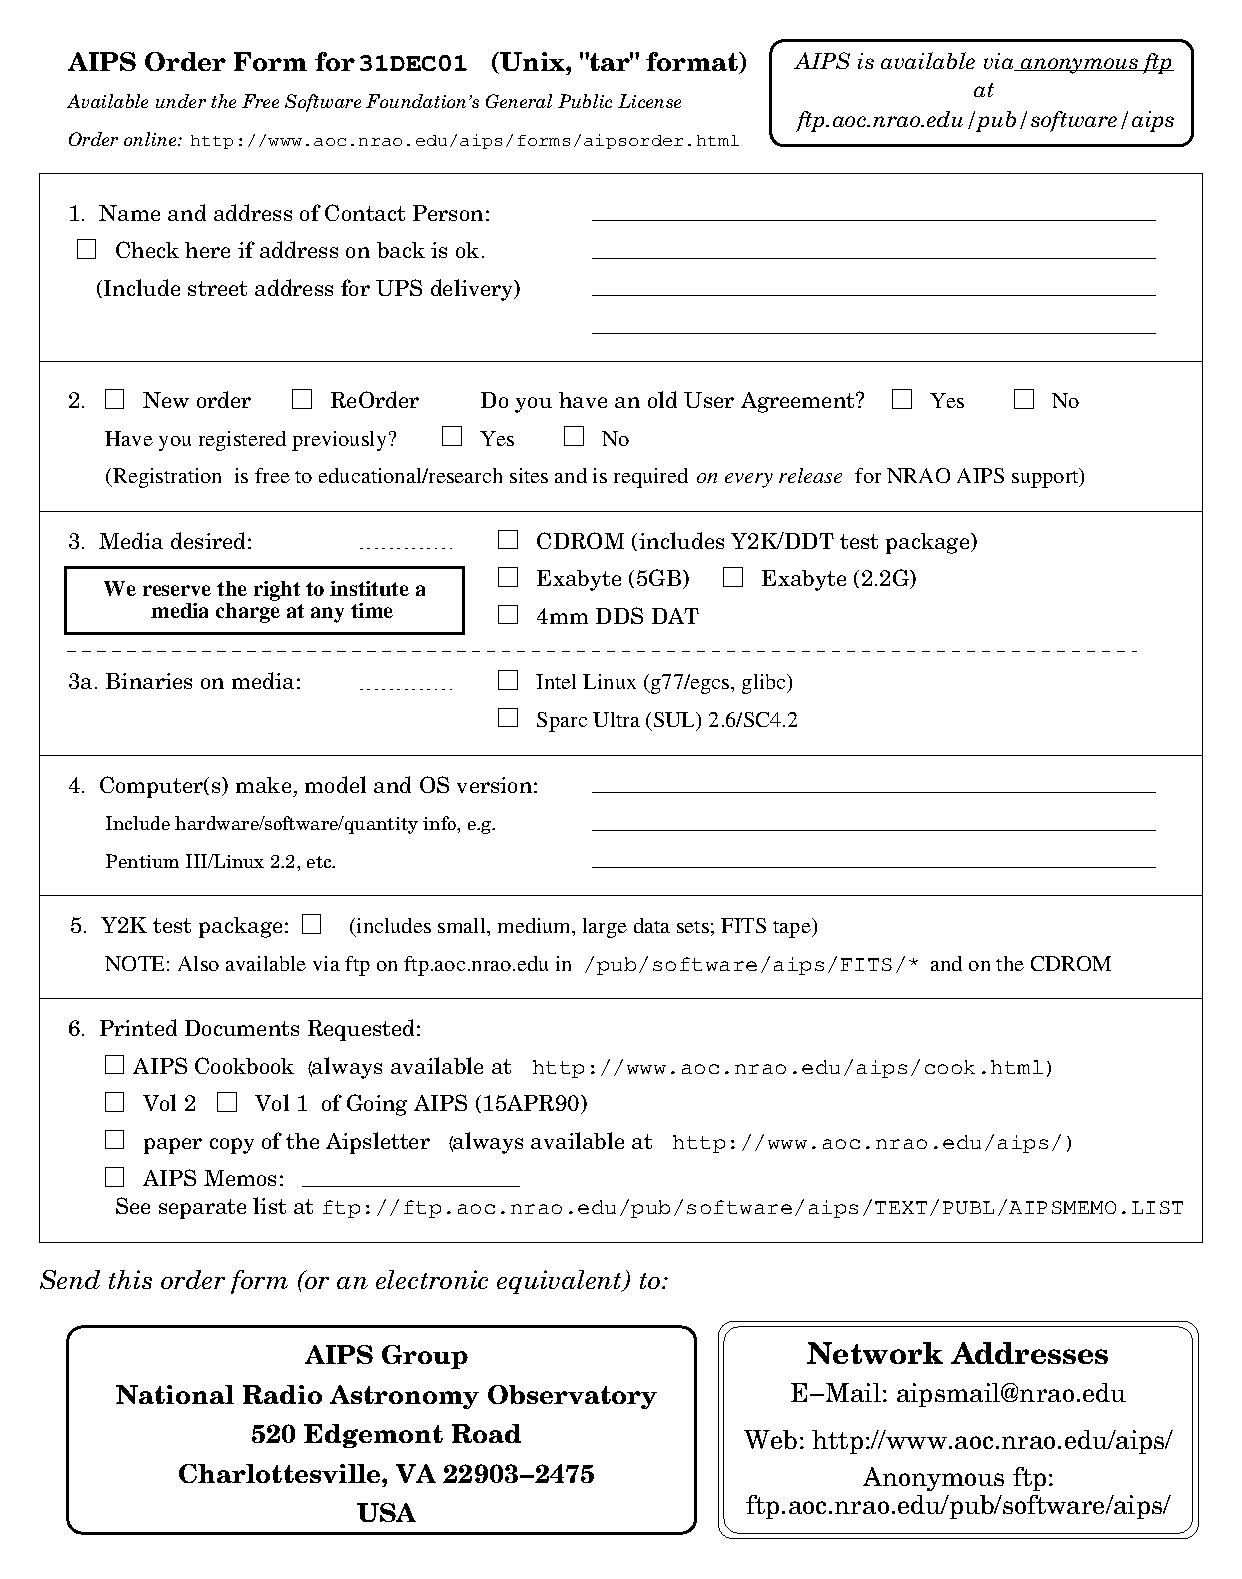
\includegraphics{FIG/AIPSORDER.PS}}}
\vfill\eject
\vbox to 4.4in{
\vspace{12pt}
%\centerline{\rotatebox{-90}{\resizebox{!}{3.5in}{%
%\includegraphics{FIG/Mandrill.color.plt}}}}
\centerline{\resizebox{!}{3.5in}{\includegraphics{FIG/Mandrill.eps}}}
\vspace{12pt}
\centerline{{\huge \tt \AIPRELEASE}}
\vspace{12pt}
\vfill}
\phantom{...}
\centerline{\resizebox{!}{!}{\includegraphics{FIG/AIPSLETS.PS}}}

\end{document}
